\documentclass{l4proj}
\begin{document}

%==============================================================================
%% METADATA
\title{Demonstrating the security of a basic cryptocurrency}
\author{Sean Horgan}
\date{September 14, 2018}

\maketitle

%==============================================================================
%% ABSTRACT
\begin{abstract}
    \vskip 0.5em
    Over the past decade, cryptocurrency has become a rapidly growing area of interest as it aims to provide a 
    decentrilised alternative to regular fiat currencies. The goal of this project is to implement a peer-based 
    cryptocurrency. It is designed to include a distributed, tamper-proof ledger, a consensus mechanism 
    for distributing transactions to all participating nodes, a mining system, and wallets for sending 
    the currency between different addresses. It also includes a test harness so that a number of nodes 
    can be created and run on a single computer in order to test the system.
\end{abstract}

%==============================================================================

% EDUCATION REUSE CONSENT FORM
% If you consent to your project being shown to future students for educational purposes
% then insert your name and the date below to  sign the education use form that appears in the front of the document. 
% You must explicitly give consent if you wish to do so.
% If you sign, your project may be included in the Hall of Fame if it scores particularly highly.
%
% Please note that you are under no obligation to sign 
% this declaration, but doing so would help future students.
%
\def\consentname {Sean Horgan} % your full name
\def\consentdate {12 November 2019} % the date you agree
%
\educationalconsent


%==============================================================================
\tableofcontents

%==============================================================================
%% Notes on formatting
%==============================================================================
% The first page, abstract and table of contents are numbered using Roman numerals and are not
% included in the page count. 
%
% From now on pages are numbered
% using Arabic numerals. Therefore, immediately after the first call to \chapter we need the call
% \pagenumbering{arabic} and this should be called once only in the document. 
%
% Do not alter the bibliography style.
%
% The first Chapter should then be on page 1. You are allowed 40 pages for a 40 credit project and 30 pages for a 
% 20 credit report. This includes everything numbered in Arabic numerals (excluding front matter) up
% to but excluding the appendices and bibliography.
%
% You must not alter text size (it is currently 10pt) or alter margins or spacing.
%
%
%==================================================================================================================================
%
% IMPORTANT
% The chapter headings here are **suggestions**. You don't have to follow this model if
% it doesn't fit your project. Every project should have an introduction and conclusion,
% however. 
%
%==================================================================================================================================
\chapter{Introduction}

% reset page numbering. Don't remove this!
\pagenumbering{arabic} 

\section{Motivation}

The concept of cryptocurrency has only emerged in the past fifteen years as an alternative to the regular,
centralised fiat currencies backed by governments around the world. In 2008 Satoshi Nakamoto, the 
founder of Bitcoin, invented the worlds first cryptocurrency providing a peer-to-peer currency
not bound to a central bank. This new currency, secured by modern cryptographic methods, is a way in
which people around the world can trade without having to send the funds via a financial institution. (REFERENCE).

This new currency ensured security to its users by implementing a distributed ledger of transactions. Bitcoin
ensured that the ledger was immutable by ensuring proof of work was given before transactions would be
added to this ledger. This invention, known as the blockchain, maintained security and prevented malicious
users from altering the system. Now the blockchain has become more than just a measure for ensuring security
in cryptocurrencies becoming useful to thousands of companies around the world and being used
in many different contexts.

Bitcoin and other cryptocurrencies are much different to current fiat currencies as they are not tied to a physical
object like a note or coin. They are also immune to inflation as the value of currency in the system is dictated
by the proof of work system. This rewards nodes for mining blocks of transactions with a small amount of the 
currency. As the currency ages this reward is reduced until eventually there won't be any more given. This places
a limit on the total amount of the currency available. 

\section{Goals}
The goal of this project is to create a secure and robust cryptocurrency from scratch. There are several key aspects
to the project that must be met in order to demonstrate a woking cryptocurrency.

The currency will be based around
a distributed ledger that is resistant to retroactive changes. It will use a concept know as proof of work,
similar to the way that Bitcoin works where nodes have to solve difficult hashing calculations in order
to add transactions to the ledger. This concept is known as mining and is a way to make sure that transactions
are added at a steady rate while providing compensation to the node as an incentive to verify the transactions the node
is trying to add are valid and acceptable.

This cryptocurrency will include wallets, allowing users to send any of their currency to another
wallet using its public key address. This will be shown in the test harness where a number of nodes and wallets 
will be created to simulate a populated network of users. A large number of emulated users will be required because on
a smaller scale cryptocurrencies do not work perfectly and are succeptable to double-spending attacks where users
can spend more money than they own. The test harness should simulate a large active network by randomly creating
transactions from user to user to then be added to the blockchain once the nodes have shown proof of work using 
the mining mechanism.

\section{Dissertation Outline}
The following dissertaiton is split into seven chapters as described below:
\begin{itemize}
    \item
        \textbf{Chapter 2} gives insight into the original Bitcoin paper and other features of cryptocurrencies
        created in the past.
    \item
        \textbf{Chapter 3} discusses the requirements gathering and analysis stage where the functionality
        of the project was decided.
    \item
        \textbf{Chapter 4} presents the way in which the cryptocurrency was designed, from the architecture of the blocks
        to the verification of transactions.
    \item
        \textbf{Chapter 5} highlights the way in which the projects was implemented, discussing the specific tools and 
        technologies used to create a secure cryptocurrency.
    \item
        \textbf{Chapter 6} discusses the evaluation of the projects. This shows how well the requirements were met, the
        performance of the system, and unit testing.
    \item
        \textbf{Chapter 7} concludes the project, summarising the project and reflecting on its execution. Here we also
        outline any future work that could be accomplished.
\end{itemize}


%==================================================================================================================================
\chapter{Background}
In this chapter we will discuss the background of the project. This will be presented by looking at the relevant research done by 
others that has similar goals to this project. We will also examine other cryptocurrencies created in the past that have aided 
in the completion of this project.


\section{Bitcoin white paper}
The first cryptocurrency to be created was Bitcoin. It was first presented in 2008 by Satoshi Nakamoto in the Bitcoin White Paper
titled "Bitcoin: A Peer-to-Peer Electronic Cash System". The concise nine page article defines Nakamoto's method of preventing
double-spending attacks in a peer-to-peer currency without the need for a third party like a financial institution to 
act as a middle man. The creater of Bitcoin wanted to avoid the use of a centralised mint as it can be seen as a single 
point of failure through which every transaction must be routed. This places the whole trust of the network on the middle 
man and the company running this mint.  Bitcoin avoids the need for a centralised middleman utilising modern cryptographic 
methods and technologies. This paper outlines the requirements for a functional cryptocurrency and as such was instrumental 
in guiding this project.

Below the main funtionality described in the Bitcoin white paper will be presented.


\subsection{Transactions}
The primary component of a cryptocurrency is a transaction between two users. In bitcoin this is described as being "a
chain of digital signatures" (REFERENCE). In this sense, a transaction is just a way of showing that ownership of the coin has
passed from the sender's address to the recipient's address. Bitcoin ensures the immutability of these transactions
by making the sender generate a hash of the previous transaction combined with the public key, equivalent to the address,
of the recipient. This means that the recipient can then verify the transaction using their own key and the transaction
is confirmed as valid.

One issue with this method is that the recipient can validate that the transaction is correct but it cannot ensure
that the sender is not double-spending the coin. This means the recipient cannot prevent the sender from also sending the 
same coin to another user. As Bitcoin was inteded to be a peer-to-peer currency with no centralised mint validating
all transactions and making sure there are no double spends, it is vital that there be some cryptographic method of
preventing these exploits.


\subsection{Blockchain}
The way Bitcoin achieves this validation without the need for a middleman is through the invention of the blockchain.
The blockchain is described as a timestamp server which works by taking the hash of a block of data and publically
announcing this hash. This proves that the data exists at that time. Then the next block of data can include the
previous block's hash in it's own hash proving that both of these blocks of data existed at that time. This creates 
a chain of blocks which prove the order and time of creation.

This chain of blocks is extremely secure as it also protects against retroactive attacks. If a malicious user tries
to go back and alter a transaction in the blockchain then this would alter the hash of that block rendering it invalid,
this would then alter the next block's hash as each block's hash is a calculation using the hash of the previous block.
This would cascade through the whole blockchain invalidating every block from the point of the malicious change. The 
network would then recognise this chain is invalid and switch to a valid chain rendering the action of the malicious
user pointless.

\subsection{Consensus}
In order for the whole system of users to work, all nodes must agree on what is the correct blockchain to be using and
which blocks of transactions are to be added to the blockchain every time. This is implemented by Bitcoin using a proof of
work mechanism. This system, also known as mining, means that in order for a node to add a block to the blockchain it
must find a value that, after being hashed, results in a number starting with a certain amount of '0's. This is 
effectivly setting a computational barrier to appending a block to the blockchain. This means that a certain amount of
CPU power is neseccary to append to the blockchain. This adds security to the system as it prevents singular malicious
users from hording IP addresses in order to take control of the network as theoretically the majority of computational
power in the network will be from benevolent users.


It is easy for the nodes to decide which blockchain to add their blocks to because of CPU power
determining which blocks are added to the blockchain. They simply choose the longest blockchain as this will be
the blockchain with the most CPU power invested in it. This is secure because if an attacker were trying to alter a 
previous block they would also have to redo all the proof of work completed for every block after that in the chain.
It is infeasable as the attacker would have to complete the proof of work for these blocks extremely quickly in order
to outpace the community and become the longest chain before other nodes would start to use that blockchain.


\subsection{Blocks}
The final point relevent to this project mentioned in the Bitcoin white paper is the way that Bitcoin aimed to store
the transactions within the blocks in the blockchain. A simple method of storing these transactions in the block may
just be an unordered list. This would work as each transaction is unrelated to the other transactions in the block in
every way except perhaps the time it took place. This storage solution can be improved though by using a data structure
known as a Merkle tree (REFERENCE). This data structure is a way in which to make the process of checking block validity
more efficient. The way Merkle trees work is by having every leaf node be the hash of the transaction it represents 
and every branch node is the hash of its two child nodes . This builds up a chain of hashes similar to the blockchain.
This means that in order for a node to check that a block is valid it only needs to check the root hash of the block as
if there were any altered transactions within the block that would have an avalanche effect up through the hashes
ultimately changing the root hash of the whole block.

Another benifit that the paper mentions of storing the transaction within the block this way is that it can lessen
the storage space needed to store each block. As the blocks can be validated using only their main hash. Nodes do 
not need to store every single transaction in the blockchain in order to confirm transactions relevent to itself.
Instead it can just store the main block hashes and save a large amount of storage. As Bitcoin becomes more and
more popular this is a significant storage space saving as the number of transactions grows larger and larger.

\begin{figure}
    \centering
    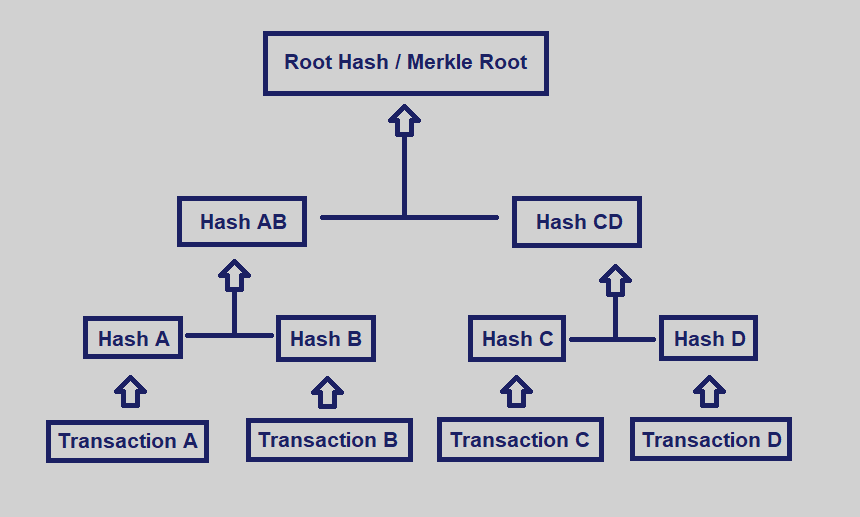
\includegraphics[width=0.7\linewidth]{images/merkle-tree.png}    

    \caption{
        The Merkle tree structure within a block of transactions. Transactions are hashed together as leaf nodes
        and repeated all the way up the tree to the main hash of the block, known as the Merkle root.
    }

    % use the notation fig:name to cross reference a figure
    \label{fig:merkle}
\end{figure}

\section{Bitcoin and Cryptocurrency Technologies}
A large source of the information used to plan this project and choose the relevant technologies to include was the
book \emph{Bitcoin and Cryptocurrency Technologies} by Narayanan et al. This provided a more in depth disscussion
about the intricacies of the structures needed for the project. The book also gave good information about cryptocurrencies
that were not Bitcoin which gave a bigger picture and provided options for doing things differently or ways to 
exclude areas of bitcoin that would not be relevant in the project.

\subsection{Flooding}
%**
One of the key topics described in the book was the way for the nodes in the network to reach a consensus. This happens
multiple times during the running of a network. *** Once when nodes must identify and decide on which blockchain to use when
alternates appear. This is described by the Bitcoin white paper by picking the longest chain and distrobuting this to 
other nodes. It also happens when a new transaction occurs between two wallets, the transaction must be sent to all
nodes in order for the nodes to include it in their blocks so they can start mining the blocks to validate the transaction 
on the blockchain.

This method of flooding is explained in the book by showing that every node has a list of nearby nodes that is created
when it joins the network. Whenever a node recieves a transaction it first performs some checks and if it passes the 
checks, the transaction is propogated to all nodes on its nearby nodes list. First, the node checks if the transaction is
valid. It runs through the blockchain and checks that the funds the sender is trying to send actually belong to the sender.
Next, the node checks that the coins are not being double-spent, meaning the same funds have not already been sent to another
address perviously. Finally, the node checks if it has already seen the transaction and if it has, it just disgards this new
transaction as the node will already have added it to a block. If the transaction passes all these test it is sent to the
nearby nodes where it is put through the same tests until eventually it is spread to every node in the network or included
in a block on the blockchain.

\subsection{Mining}
One functionality described in the book is how mining changes over time. When a node mines a block that is included in the
blockchain they recieve a small reward which is an incentive to keep the blockchain updated. As explained perviously,
mining is the process of solving a hash calculation to result in a number starting with a certain number of '0's. The number
of 0s or target range, is changed over time. In Bitcoin, once every 2016 blocks that are mined the difficulty of mining will be
altered. The way that this difficulty is altered depends on how quickly blocks were mined in the previous 2016 blocks. This
is done in order to maintain a consistant mining speed. The faster the nodes are mining blocks, the harder the difficulty
will subsequently become. As the network of users increases, the processing power increases and so the mining will happen
faster. This is also offset as over time the size of the incentive reward for successfully mining a block is lowered.
This reward system is the only way new coins are created and because of this there is a maximum to the total amount of coins
that will be in the system. This effectivly makes Bitcoin immune to inflation.

The way bitcoin automatically responds to changes in the amount of processing power and size of the network is impressive,
however will not be a useful addition to the project. As this project will run at a relativly small scale over a small
time span, it would not be utilised and would be unnecessary to include this feature.

\subsection{Bitcoin scripting}
Another major part of blockchain that the book describes is the small scripting languague that was invented specifically for
transactions which helps with the verification of transfers. This simple bitcoin scripting language is used
by nodes when mining blocks to verify that all transactions in the block are valid. Every transaction in Bitcoin is
sent with a script, most often instructing the node to compute the inputs of this transaction and the specified outputs of
previous transactions to make sure they match up correctly. Bitcoin also utilises this scripting language to inform the node
what the output should equal when the receiver tries to verify the transaction signature using their key. The book goes
into detail about the intricacies of the language but this is out of scope for this project because including this scripting language
in the project would be unnecessary as there would only be one script needed and this can be implemented without the script.


%==================================================================================================================================
\chapter{Analysis/Requirements}
In this section we outline the exact nature of the project and how we gathered these requirements in order to 
complete the goals listed previously. We also discuss any functionality or features that have deliberatley been
left out of scope.

In this project the MoSCow method was used in order to prioritise the features so that the most important attributes
were included and some of the less important ones could be left to the end of the project to be added in if there was
time to spare.

\section{Functional Requirements}
Functional requirements listed here are features that must be included in the project in order for a woking,
useable cryptocurrency to be created. Without these requirements being met it would be impossible to carry out any
useful form of evaluation.

\subsection{Must have}
\begin{itemize}
    \item As described in the goals for the project, it would not constitute a cryptocurrency if it did not include a tamper-proof
        ledger for keeping track of all transactions between users. This must be resistant to malicious retroactive alterations
        and transactions that are invalid. This means that it must also have a feature so that nodes can run through the 
        whole chain and check all transactions are valid and each block links to the previous block.

    \item The cryptocurrency must also include some form of consensus mechanism where nodes can agree upon the blockchain
        and decide which transactions to include on the blockchain. They must be able to circulate each transaction once
        it occurs and flood it to other nodes on the network.
    
    \item Before blocks can be added to the blockchain it is important to inculde proof of work so that the integrity of the 
        networks blockchain can be maintained and guided by the processing power of the whole network and not a small minority
        of harmful nodes trying to take over.
\end{itemize}

\subsection{Should have}
\begin{itemize}
    \item A feature that can help with the smooth running of the network is an incentive for nodes to mine blocks. Without this there
    is no reason for nodes to mine blocks and add to the blockchain. This is necessary as there needs to be a majority of 
    honest nodes othewise it is easy for malicious nodes to take control of the blockchain and can then add any blocks with
    which ever transactions they would like to the blockchain wether they are valid or not.
\end{itemize}


\subsection{Could have}
\begin{itemize}
    \item In Bitcoin, every 2016 blocks that are mined the difficulty of mining is changed in order to maintain the same average time
    to mine a block. This difficulty is either made harder or easier based on how quickly the nodes mined the previous blocks.
    This is not a high priority in this project as all the mining is taking place on the same computer and each node will have
    the same computational power. In theory this means that the average time for mining blocks shouldn't change.
\end{itemize}


\section{Non-Functional Requirements}
Non-functional requiremnts are features that if included will improve the way the cryptocurrency operates by increasing
speed or lowering the storage space required. These features are not imperative to the operating of the cryptocurrency
but would bring the project closer to what might be used in current cryptocurrencies in the world at the moment.

\subsection{Must have}
\begin{itemize}
    \item It is important that the way in which the transactions within blocks is efficient. The must be stored using the Merkle
    tree structure (REFERENCE). This way each transaction is a leaf node and every branch node is a hash of its two children.
    This makes it extremely efficient for checking the validity of each block as you only have to check the hash of the root
    hash.
\end{itemize}


\subsection{Should have}
\begin{itemize}
    \item The cryptocurrency should have the ability to split the balance of wallets such that if you send an amount but you only
    have an increment of the currency larger than that amount then you should be sent back the value that you overpaid by.
    For example if you start with 10 coins and you want to send 3 to another wallet you should be able to send your 10 coins
    and recieve 7 back as overpay.    
\end{itemize}

\subsection{Could have}
\begin{itemize}
    \item One feature that would save storage space would be the way in which transactions are stored in blocks. In the Merkle tree
    structure the transactions are hashed in order to speed up validation for nodes. This could be improved even more for 
    nodes. It is possible that nodes only need to store the root hash of each block in order to do their validation as the
    block hash is sufficient to check for incorrect transactions. This means each node can save a huge amount of storage space
    by only storing each blocks root hash.
\end{itemize}

\section{Chosen Limitaions}
In this section some of the limitations that have been placed on the project which would not help demonstrate the 
primary purpose of the project are presented.
\begin{itemize}
    \item One feature that has been omitted is the concept of scripting. In Bitcoin, every transaction is sent
        with a short piece of code writen in the Bitcoin scripting language. This serves the function of allowing 
        different forms of transactions like ESCROW or multi user transactions. While useful in the functionality of
        Bitcoin, this feature is not necessary in our implemtation of a cryptocurrency as there will only be a need
        for one type of transaction.
    \item Another aspect chosen to exclude is the way in which nodes work. In real cryptocurrencies if a node
        has not been active in mining or creating transactions, after a specified amount of time the node will expire
        meaning other nearby nodes will cease to send transactions to this node. This effectivly removes the node from
        the network. This functionality is useful in keeping the list of nodes exclusive to active nodes and saves
        collective processing power for the whole network. In the project's implementation this would be unnecessary as a fixed
        number of nodes will be created for demonstration perposes.
\end{itemize}

%==================================================================================================================================
\chapter{Design}
In this section the decisions that were made when designing the project in order to meet the requirements
that have been laid out in the previous section are disscussed. The discussion will include the approach taken when
choosing one particular design instead of another and why those choices were made.

\section{Overview}
The main aspects of the design process that needed to be addressed were transactions, the blockchain, and
the consensus mechanism. It was also necessary to decide how all of these data structures would be linked together and
how the overall process of sending currency from one wallet to another would work between these structures.

%Maybe a system diagram showing how the structures interact
%Mention how there can be multiple blockchains

\section{Transactions}
%Structure and values
A transaction object is the basic building block of the whole cryptocurrency. This means that it must be designed 
to be secure and robust. Transactions should contain metadata that is able to identify and validate itself when
recieved and also contain the necessary information such as the amount of currency being sent in that transaction.

\subsection{Inputs and Outputs}
In order for a user to send some currency to another user they first have to have a sufficient amount themselves. The
way this condition was enforced was through the use of Transaction Inputs and Outputs. When a transaction is
sent, the value of that transaction (amount of currency it is attempting to send), is a collection of inputs. These inputs
are made up of the outputs of previous transactions that have been addresed to the user. This means that the process of
checking a user's balance would involve going through the blockchain adding up all the transaction outputs that
are addressed to that particular user and not already spent. This concept will be explained in more detail in the Blockchain section.

%Diagram of a transaction
\begin{figure}[!ht]
    \centering
    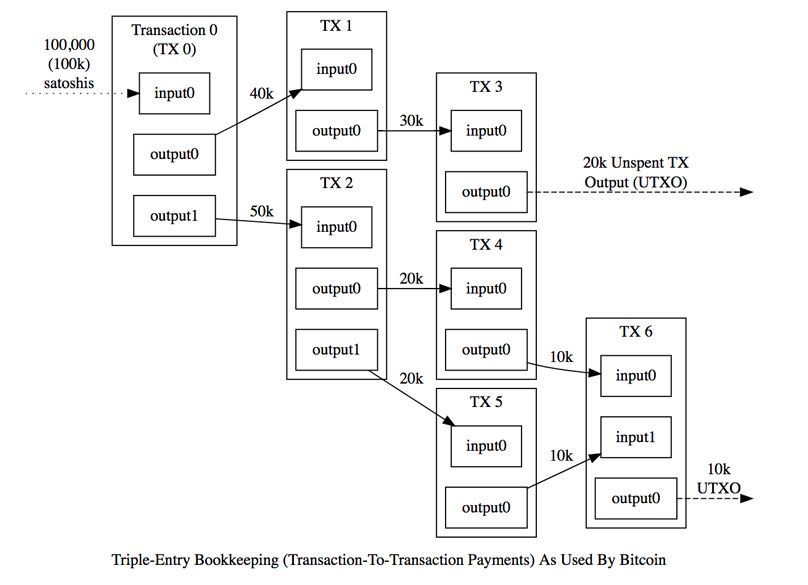
\includegraphics[width=1\linewidth]{images/utxo-model.jpg}    

    \caption{
        This diagram shows the process of transactions. Transactions require inputs to send value. These inputs come from
        the outputs of previous transactions. These transactions then produce more transaction outputs which conntinue
        the chain. This is the process Bitcoin uses and is the same one that will be used in this project.
    }

    % use the notation fig:name to cross reference a figure
    \label{fig:transaction} 
\end{figure}

\subsection{Process and Checks}
%signatures
A key functionality of a transaction is it's ability to generate a signature for itself using the values
from the various metadata it contains. It also has to be able to verify that this signature is valid.

%Process transaction
When a transaction is created it has to be processed before it is considered valid and added to a block and subsequently
the blockchain. This is done using a series of checks. The first check that the transaction makes is that the
signature is valid. This is paramount as it is one of the base functions that maintain the security of the 
cryptocurrency. Without this signature check it may be possible for one user to spoof the origin of a transaction
and send someone else's currency to themselves. The next step is to add up all the transaction inputs
and make sure that this is greater than or equal to the value of the transaction.

Once these checks have been completed it is time to execute the transaction. The way this is achieved is by
creating a new Transaction Output addressed to the recipient using the value of the transaction. It is important
that the previous transaction inputs are then removed as otherwise they would still be valid for the user to send
running the risk of double spend attacks. This is covered in more detail in the Blockchain section.

%Overpay
\subsection{Overpay}
In a real environment it is common that the ammount a user is trying to send is not equal to the value of one of
the transactions they have recieved in the past. For example, if a user recieves a transaction of 10 it is likely
that the next time they want to pay someone they may want to only spend 5. This issue is solved by the concept of
overpay. In this design, when a user is sending a value to a recipient which is not equal to the transaction
input they are expending, the transaction processing creates two transaction outputs. The first sends the value
of the transaction to the recipient and the second sends the transaction input value minus the transaction value
back to the sender. This ensures that the transaction input is used up but the sender is not out of pocket.

%Coin creation
\subsection{Coin Creation}
When a transaction is created it can be one of two types. The first type is that of a normal transaction which would take place
between one wallet and another. The second type is that of coin creation. A transaction can be created with the 
coin creation flag which means that the inputs to the transaction would not contain anything but the transaction
would still be considered valid. This would only occur in the scenario like the very first transaction for the entire
cryptocurrency or the more frequent scenario which happens when a block is mined. To keep the system of consensus 
running there has to be an incentive for mining blocks. When a node mines a block they are rewarded with a small
amount of the currency which does not come from any particular user, instead this comes from a transaction with the
coin creation flag. After the initial creation of the network this is the only case where new currency will be
minted.

\section{Blockchain}
The second major feature of the project to design is the Blockchain. This chain of blocks needs to be robust in
the sense that a malicious user cannot benidit by altering any previous transactions in the ledger. It must
also be an accurate ledger containing every transaction exchanged to date. The way this blockchain was created was
by first collating a group of transactions into blocks. Then each block would create a signature hash which would
be a combination of all the transactions in the block. Then, in order to create an irreversible and immutable chain
of these blocks, the hash of each block is concatenated with the hash of the previous block in the chain [\ref{fig:blockchainDiagram}]. This means
any change to a transaction would cascade through each hash in each block and ultimately affect everything in the
chain. This means that it is easy for any node to check that the blockchain is valid using a simple and fast check.

%Blockchain diagram
\begin{figure}[!ht]
    \centering
    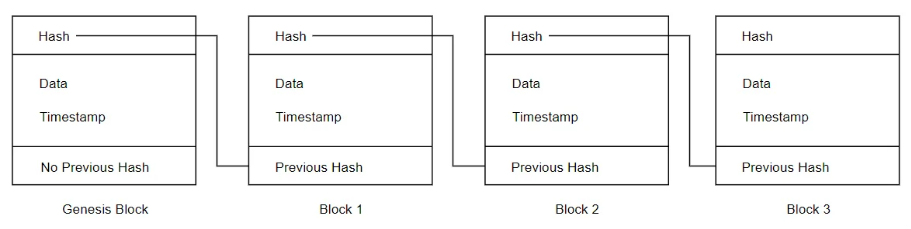
\includegraphics[width=1\linewidth]{images/blockchaindiagram.png}    

    \caption{
        This figure shows how the blockchain works by having the previous block's hash fed into the next
        block's hash in order to create a chain.
    }

    % use the notation fig:name to cross reference a figure
    \label{fig:blockchainDiagram} 
\end{figure}

\subsection{UTXOs}
The strategy of utilising Transaction inputs and transaction Outputs means that it is vital that the Blockchain
keeps track of the transaction outputs. When a user sends currency to another user, it is vital that the previous 
transaction output that the user has now spent, is removed. This is necessary for a few reasons, 
firstly if a user wants to find out how much currency they own they need to sum all the transaction outputs that 
are addressed to them. If the transactions are not tracked by removing transactions that are already spent, the 
user may be able to spend more than they own using double spending attacks.

This leads to the concept of an Unspent Transaction Output list (UTXO). This list is a structure tied to the blockchain
that stores all the transaction outputs that have not been spent as inputs by a tranasction. When they are used 
the transaction processing stage removes that output from the UTXO list and adds the new output to the list.
It is important to note that this is not a list of new transaction ouputs as that would not be secure outside the
blockchain and would be vulnerable to attack. It is simply a way of listing the transactions already added to the
blockchain. When a transaction is processed it goes through the new block and updates the UTXO list by recreating 
it. This maintains security and prevents malicious users from attacking the system this way.

\subsection{Block Structure}
%reference the previous diagram
The way the storage of transactions inside blocks was decided was using the same method utilised by Bitcoin using
Merkle trees. As mentioned earlier in this paper, a Merkle tree is a type of binary tree where each leaf node
is a transaction and each branch node is a hash of its two children. It was decided this would be the most effective
way of storing the transaction for this method as it would allow efficient and cheap validity checks for nodes
when testing the correctness of the blockchain. As this project is being designed to run on a test harness on one
machine it is important that the nodes be able to perform checks as quickly as possible.

%block size
Another important factor was the number of transactions to include in a block. The larger this number is, the
longer it will take to fill up with transactions and so the longer it will take I decided to keep the 
number of transactions in blocks relativly small in order to progress through the cryptocurrency lifecycle
more quickly and demonstrate all features.

\section{Consensus}
This final section dicusses the way in which the system was designed in order that all nodes communicate correctly and
that they all maintain an up-to-date copy of the blockchain. It also explains the decision to 
use one particular method of mining instead of alternatives.

\subsection{Proof of Work vs Proof of Stake}
In order for the network to function correctly, a consensus must be achieved by all the nodes. They need to agree
on what the correct blockchain is so they can add to it and they must also keep a consistant list of all the 
transactions yet to be included on the chain. It is vital that this consensus is achieved by nodes that are not
malicious or compromised and that the consensus they come to is proposed by an honest node to avoid attackers
taking over the blockchain. 

There are two common methods of distributed consensus methods. Proof of Work and Proof of Stake. These methods
are a way for nodes to prove that they are not malicious and are simply trying to honestly contribute to the
network. These concepts are not limited to cryptocurrencies and have many other applications in the world that 
have been researched by others [1,2]. The main idea behind these methods is tying the task of adding blocks to the 
blockchain to a reasouce that cannot be monopolised and as such the whole network cannot be controlled by a 
singular entity. Each method aims to achieve this in a different way by using different resources.

\subsubsection{Proof of Work}
This approach is the method that Bitcoin and most other cryptocurrencies use today. The resource it uses to 
ensure honesty is computational power. This means that in order to create a new block, a node has to demonstrate
that it has expended a certain amount of computational power. The way this is achieved is using hash calculations. 
This works by having a node take the previous block's
hash and the hash of the current block concatenated together with a number known as a nonce, resulting in a number
that falls within a specific target range. Nodes must go through incrementing the nonce in order to find the 
correct value that will satisfy the requirement. The size of the target range influences how hard and so how long
it will take for nodes to find. Once a node has found a nonce that results in a value inside the target range
they have proven that they have used compuational power and are entitled to add to the blockchain.

\subsubsection{Proof of Stake}
Much like the proof of work method, proof of stake is essentially assinging nodes the power to vote on what the
blockchain should be. The more of a resouce a node has, the more voting power it has. Proof of Stake is different
to Proof of Work as instead of tying voting power to computational power, it ties voting power to the amount
of currency a node holds. This means that the nodes with the most currency hold the most power to decide what the
blockchain will look like. In practice this means that these rich nodes will more often be selected to add a new
block to the chain. This methods has many advantages over the proof of work concept. This would significantly
reduce the environmental impact of the whole currency as there would be little to no mining taking place and so
there would be no groups of computers solving calculations indefinitely. This has the added benifit that
it would lower the chance that the network would become more centralised by mining companies. This method also
avoids the risk of a majority of malicious nodes aiming to destroy the currency. As any user holding any amount
of the currency is essentially a stakeholder in the network, any node that achieves a majority of the currency 
would have the ability to alter the course of the blockchain. With this method however, it would be in the best
interest of the majority stakeholder of the currency to perform honest actions as that would increase the value
of their currency.

In this project I have chosen to use the Proof of Work system as despite the real world benefits, like environmental
welfare, the proof of stake method does not present advantages when using a scale such as that being implemented
in this project. It would be more beneficial to show the proof of work system as mining would demonstrate the
functionality of the system better.

In this cryptocurrency the target range will be a number that begins with a certain
ammount of 0s. This means I have the ability to adjust the difficulty of the mining process by increasing
or decreasing the number of 0s in the target range. The more 0s required means that the final value must be more
specific and as such will take longer to find. I have decided that for this cryptocurrency the difficulty of mining
will remain low as processing power comes at a premium for one computer running multiple nodes.

\subsection{Nodes}
%Nearby nodes
In order for nodes to be able to communicate the details of transactions and the correct blockchain to use,
they first have to be able to identify and keep a list of nodes that are nearby in the network. This does not
necessarily mean geograpihcally nearby but in practice it is most likely nodes created most recently.
The way nodes are designed in this project is that a node is created with a seed node. Upon creation, nodes
query the seed node in order to obtain a list of nearby nodes, these nodes are selected randomly in order
to avoid every node's nearby list containing the same subset of the network.

%Transaction Flooding
\subsubsection{Transaction Flooding}
In order for nodes to mine blocks, they first have to know what transactions to include in the blocks. To do
this they need to know what transactions have occurred that are not currently included on the blockchain. This
is achieved by transaction flooding. When a transaction is created by a wallet it is sent to the node that the
wallet is associated with. This node then performs some checks on the transaction. The initial check is to make
sure that the transaction fits with the blockchain. It runs through all the inputs that the transaction claims
to be spending and makes sure that they line up with transaction outputs listed on the UTXO to make sure they
exist and haven't already been spent. The second check is to see if the transaction has already been seen by
the node if so it moves on without adding it to the block it is trying to create. If the transaction passes
these tests then the node adds it to the block it is planning to mine and then sends the transactions on to all
other nodes on its list of nearby nodes. Nodes recieving transactions like this from other nodes will perform the
same checks and then decide whether to pass on the transaction again. This way the transaction should be flooded
through the whole network and be eligable to be added to any block.

\subsection{Wallets}
%Something about wallets, maybe the overall process of sending coins
The design for wallets in this project is that every transaction must be tied to a wallet and every wallet
must be created from a node. This way, when a wallet creates a transaction it is automatically sent to the
associated node and can be flooded to the network. Each wallet has a public key which is used as the address
for which currency can be sent to and a private key which is used to verify each transaction. The wallets 
keep track of their own currency by running through the blockchain and adding up every transaction output
that is addressed to themselves. Even if a wallet spends some currency and then tries to spend the same
currency before the previous transaction is added to the blockchain it will be caught by the nodes before the
transaction will be flooded to prevent double spending attacks.

\section{Test Harness}
%Describing how the whole process works together
%Can include diagram showing main program flow
The final stage to designing the project was deciding how all of these features of the currency could be shown
and how the security could be effectivly presented. To meet the requiremnets specification it would mean developing
a test harness that could generate multiple nodes and simulate a real network of sending transactions back and 
forth between wallets in order to demonstrate the building of blocks and the blockchain. All while Demonstrating
the prevention of doubling spending and other attacks. 

\section{Chosing a Programming Language}
%Explain why object oriented programming was necessary 
%Explain why java for security packages etc
In order to decide what language we would use for this project it was best to look at how the project was designed
and then narrow it down to the most suitable contenders. The way in which this cryptocurrency was designed was 
utilising many different objects and structures, transactions, blocks, and the blockchain. This made it clear that 
the best choice of language for the project would be an object-oriented programming language. This narrowed down
the playing field to \textit{Java} or \textit{C\#}. From this it was decided that \textit{Java} would be the best 
option as it includes security packages which would be invaluble for implementing core features like signatures and 
public/private key verification.

\section{Summary}
This section outlines the way that the project was designed in order to meet the functional and non-functional 
requirements set out in the previous section. It also covers why some decisions were made like choosing one design 
over another.

%==================================================================================================================================
\chapter{Implementation}
This section of the paper will go in depth into the technical construction and implementation of the cryptocurrency.
This will start with describing the software development process used during construction and then how the different
aspects of the project were created and joined to deliver the finished product. This section will also examine the 
technical achievements made and how any problems that came to light were tackled.

%Challanges and how they were overcome
%What did you do to implement this idea, and what technical achievements did you make?
%You can't talk about everything. Cover the high level first, then cover important, relevant or impressive details.

\section{Software Engineering Practices}
In order to create this cryptocurrencies it was important to have a solid software development process and an
aim to stick to the different practices.

\subsection{Version Control}
It was decided that the method of version control to be used would be Git. Making use of the GitHub website to 
host the project repository online. This allowed for the addition of code from different computers during the
development stages. This project made use of the branching feature of git in order to keep the project organised.
Every new feature/element that was added was designated a new branch and once complete was merged back into the
main development branch. Only at the end of the project was everything merged back into the master branch. This
was decided as the master branch is always supposed to keep a working copy of the software but this working copy
would not exist until the very end of the project as all the features had to be completed in order to work together
correctly. This was also the reason why the decision to not make use of continuous integration was made. It was
much faster and easier to run small tests and log outputs locally rather than make use of \textit{TravisCI} or an 
alternative.

GitHub was an incredibly important website to the construction of this project as it allowed the ability to keep
track of the completion of each feature using issues and milestones. Each feature and even small bugs were assigned
an issue [\ref{fig:issues}] and then those issues were assigned to one of the milestones [\ref{fig:milestones}]. 
This made it easy to prioritise each feature and keep on track with what needed to be done. The ritual of creating
an issue when a feature or problem is identified and then closing the issue when it is dealt with was important to 
the smooth development process.

%Maybe include committing and pushing.

% Issues Screenshot
\begin{figure}[!ht]
    \centering
    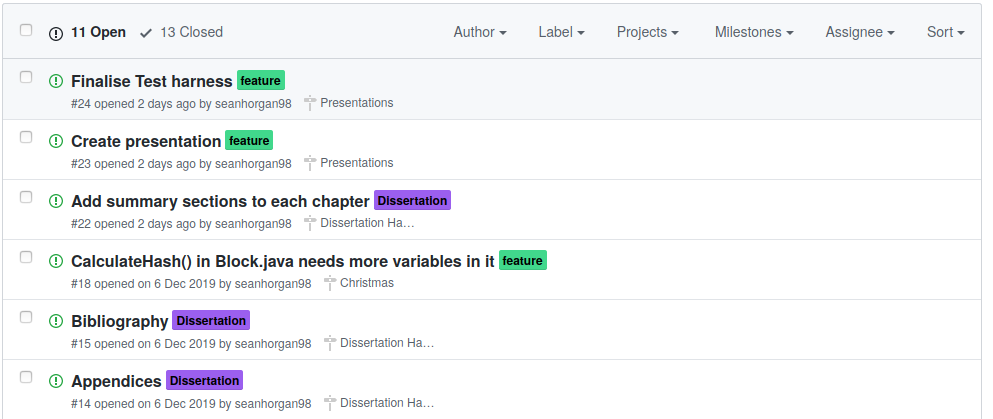
\includegraphics[width=1\linewidth]{images/issues.png}    

    \caption{
        A view of the main issue tracking board on GitHub. Making it easy to keep track of state of the project
        and what is still left to be completed.
    }

    % use the notation fig:name to cross reference a figure
    \label{fig:issues} 
\end{figure}
\vspace{10cm}

% Milestones screenshot
\begin{figure}[!ht]
    \centering
    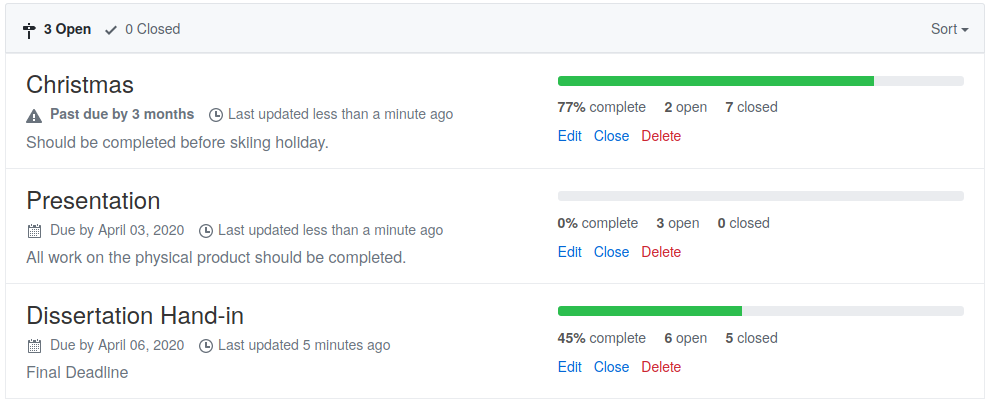
\includegraphics[width=1\linewidth]{images/milestones.png}    

    \caption{
        The main milestone board on GitHub showing the dates that each feature need to be completed by and
        allows for easy prioritisation of issues.
    }

    % use the notation fig:name to cross reference a figure
    \label{fig:milestones} 
\end{figure}

\section{Project Strucutre}
%Separation into classes and the string util class(will be talked about later), main
As this project lended itself to using an object oriented approach it made sense to separate the project into
Java class filed for each object. These object would then be able to interact together by calling functions
of other classes throughout the process. This left the main class which was used to host the test harness by
instantiating all the objects and simulating many nodes and transactions.

%Project structure diagram

\section{Java security (String Util)}
%Signatures
As described before, one of the reasons for choosing Java as a programming language was so that I could make use
of the security packages that are included in the language. These packages were utilised mainly in a utility class created
called StringUtil.java. The purpose of this class was to provide three functions that would be used in other aspects
of the program. 
%Maybe describe hashing more in depth to emphasise security
\subsubsection{ApplySha256}
The first function applySha256() takes in a string input and apply the SHA256 encryption
algorithm to that string and return the result. This function was used all throughout the program for generating
the hash values for objects. When an object like a transaction or a block is created, it takes all the metadata that
it is created with and feeds them into this StringUtil function which returns the hash value. This essentially gives
a unique identifier to every instance of each object. This function is the core of what keeps each block from being
tampered with retroactivly as the hash identifier created by this function would change if any of the metadata from
the block would change.

%Show hashing equation
%Explain more indepth how this was used for almost everything to hash stuff

\subsubsection{ApplyECDSASig}
The second function, called applyECDSASig(), is a function that takes in a key and a string as inputs and
applies the Elliptic Curve Digital Signature Algorithm (ECDSA) to the string using the key. This is used to encrypt a string
of data using a private key so that it may only be unencrypted using the public key that is associated with the private
key. This function is another cornerstone of the security for the project as it used in this project when generating
a digital signature for each transaction. When a transaction is created by a wallet it generates a signature for
itself using the private key of the sender and data which consists of the metadata of the transaction like its value
and the wallets involved. 

\subsubsection{VerifyECDSASig}
The third function of this class is the counterpart to the applyECDSASig() function called verifyECDSASig(). This 
function takes in a public key, a string of data, and a digital signature. It takes these inputs and using the Java
security packages verifies that the signature is valid for the data using the public key. This function is used
when recipients of a transaction are trying to redeem the value sent to them. When a transaction is being processed
by a node to be put into a block it attempts to verify the signature that was created by the sender. It feeds the metadata
of the transaction, the public key of the recipient, and the digital signature of the transaction into the verifyECDSASig()
function and if it does not return true then the transaction does not process and is disregarded.

These functions utilise a clever part of cryptography where transactions that are signed by the private key of the
sender can be verified by anyone that they come from that specific user by using their public key. This means that 
transactions cannot pretend to be sent by anyone as each user should only have access to their own private key.

\section{Data Structures}
One of the main challanges with this project was deciding what data stuctures should be used for each object and
how all of these objects were able to interact. These decisions were vital to being able to correctly implement
all of the requirements. This section goes into detail which structures were chosen and why these were the best
choices.

\subsection{The blockchain}
%Why blockchain is an arraylist
In this implementation of a cryptocurrency the blockchain is represented with an ArrayList data structure cointaining
all of the blocks [\ref{lst:blockchainDefinition}]. This was a simple and easy way to store the blocks as the actual data structure did not need to
have any specific security. All the security is created around this structure so all that was needed was a simple 
strucutre to store a list of blocks that was easy to work with. 



\subsection{The UTXOs}
%UTXO hashmap
In order to store the UTXOs it was important that a data structure was used such that the actual transaction
object could be tied to the transaction that created that output. This meant making use of one of Java's HashMaps
[\ref{lst:blockchainDefinition}]. Every time a transaction is processed by a node the outputs that are created 
along with the ID of the transaction are appended to the UTXO map. After this the process transaction function 
removes any transaction inputs that have been consumed in the process of the transaction.

\begin{lstlisting}[language=java, float, caption={This figure shows the definitions for the blockchain and also 
    the UTXO maps. The blockchain is an ArrayList created with one starting block acting as a genesis block. The 
    UTXO map is a HashMap mapping the transaction id to the transaction output created from each transaction.},
    label=lst:blockchainDefinition]
    public ArrayList<Block> blockChain = new ArrayList<Block>(1);
    public static Map<String,TransactionOutput> UTXOs = new HashMap<String,TransactionOutput>();
\end{lstlisting}

\subsection{Blocks}
Similar to the way the blockchain stores all of the blocks, the blocks store their respective transactions 
using an ArrayList as well. This allowed for easy manipulation of the transactions within to help the process of
building the Merkle tree structure.

One technical challange that needed to be overcome was how the Block class would organise all its transactions
into the Merkle tree structure. This was implemented by first taking a copy of the list of transactions in the
block to work on. Then, using a utility function, it would loop through the list and every two transactions it 
adds the combined hash to a new list. This is repeated until only one hash is left which is known as the root 
hash of the block. This would result in a structure identical to the one described previously in this paper
[\ref{fig:merkle}].

%Maybe add more depth to explain this better.

The Block class also contained a function dedicated to returning the Merkle root of the block which saves 
significant time when nodes are traversing the blockchain to make sure it is valid.

\section{Testing}
%How the unit tests work
As one of the main aspects of this project is the security of the cryptocurrency, it is important to include
thourough unit tests throughout the project to make sure that the features they are testing are working correctly.
It is not only the unit tests that matter however, there are also tests that are run during normal functionality
like the tests that are run when nodes are deciding how to handle incomming transactions from other nodes in the
network. This section covers how these tests were constructed and any challanges that had to be overcome in order
to keep the network running.

\subsection{Blockchain Tests}
%Checking the blockchain is valid by going through each block hash by hash
The main test used on the blockchain had the goal of making sure that the whole blockchain was valid. This meant
ensuring every block in this particular blockchain had the correct hash and linked to the correct hash after it.
This was achieved in practive by looping over the whole blockchain and first calculating a new hash using the 
transactions within for the current block and checking that it was equal to the hash that is saved in the 
blockchain. This test would also run through and make sure that each block in the chain has the correct hash
stored of the previous block in the chain ensuring continuity.

This test is vital to the security of the whole network and is run by every node when joining the network,
mining for a new block, or when switching from one blockchain to another longer blockchain.

\subsection{Node Test}
%Add more depth to the transaction validation parts
The tests that each node run are in relation to dealing with new transactions when they are flooded through
the network from other nodes. This is covered breifly in previous sections but here I will present more depth
on the implementation of these tests.

\subsubsection{Valid Transaction}
This test checks whether the transaction is a valid construction. This is essentially checking that all the inputs
correctly match up to previous outputs on the blockchain. This test achieves this by looping through each transaction
input for this transaction and checking the parent transaction ID attribute for that input matches with a transaction
on the current blockchain that produces a transaction output that matches. If no matching transaction is found
then the transaction is disregarded from the block the node is building and not sent to any other nodes. This test
carried out across the network stops the transaction from entering the blockchain.

\subsubsection{Are Outputs Spent?}
The second test is to remove the chance of users committing a double spending attack. This is done by checking
that the outputs that are being consumed for this transaction have not already been spent. The test achieves this
by running throught the the blockchain and checking if any transactions are using the same transaction outputs 
as the current transaction is trying to use. If so the transaction is removed and not spread further through
the network.

\subsubsection{Has Transaction already been seen?}
This one is simple as it simply runs through the exsisting transactions in the block it is building up and
checks if the current transaction matches any of them. If they do then the transaction is disregarded from the
block and not sent to any other nodes.

\section{Nearby Nodes Algorithm}
%Nearby Nodes algorithm
One key aspect to the network is the process of node creation. As briefly discussed earlier in the paper, nodes
do not carry an up to date list of all nodes in the network at all times. This would be bloated and unnecessary.
Instead, nodes keep a small list of nodes that are topographically nearby on the network. In practice these nearby
nodes tend to be nodes that are created within similar time frames as each other. When a node is created it is
paired with an already existing node called a seed node. This way, every time a new node is created it can query
its seed node to find new nodes on the network. This algorithm for building a nodes nearby nodes list is important
as if a node were to simply copy the nearby nodes list of its seed node then all nodes would be created with the
same list and it would be impossible for transactions being flooded through the network to reach every node. Instead
a recursive method is used. The algorithm sets up a loop to run until the node's nearby nodes list is full
[\ref{alg:nearbyNodes}]. Each iteration it gets a random node in the seed node's nearby nodes list and checks if 
the current node already contains that node in its list. If so it ignores it and moves on. If it has not seen 
that node then it is added to the list and the loop moves on to the next iteration. At the end it is important 
that the node adds itself to its list of nearby nodes. This seems redundant but it is necessary in order for 
future nodes to be able to select that node to be part of their lists.

\section{Switching Blockchains}
Another technical challange that had to be achieved was the ability for nodes to switch from one blockchain
to another. In real world cryptocurrencies this mainly happens when one blockchain is longer than another or
when one blockchain becomes invalid. A blockchain could become invalid if a transaction of block is changed 
causing the chain of hashs to become invalid. In the case of this blockchain this should not happen as we can
control whether nodes are honest and not trying to alter previous transactions in the blockchain.

Nodes in this project are able to decide which blockchain to use. They hold a variable called currentblockchain
which they perform all their functions on like mining blocks. If they are notified about a blockchain that is
longer than their current blockchain, they are able to switch to that blockchain. Before they switch they must 
make sure that the blockchain is valid however, this is done by calling the validateChain test described previously
on the new chain. This switching feature ensures that all nodes are currently working on the longest available
valid blockchain. Any transactions that have been added to a blockchain that is no longer being used by the network
will not be counted until it is added to the new chain. This means people will not be able to double spend currency
that is sent on two different blockchains.

\section{Sending currency}
The process of sending currency from one wallet to another is more complicated than just creating a new transaction
object. In this project, transactions are created by a wallet object by calling its sendFunds() method with
the public key of the recipient and the value of currency you wish to send. This function then has the job of
creating the new transaction object and sending that transaction to the network of nodes.

The method achieves this by first checking the wallet has enough currency to be able to send the desired value.
This is done by scanning through the blockchain and matching any transaction outputs that are addressed to this 
wallet. These are then added up to find the total balance of the wallet. These transaction outputs are saved to a
local hashmap variable to be used in the next step.

The next step is to create a list of transaction inputs that will be used to generate the transaction object.
This list is populated by running through all the UTXOs that are address to this user which were discovered in 
the previous step. Each iteration the values of these transaction outputs are added to a total and a new 
transaction input object is created with the same value as the output object. This new input object is added
to the arraylist created earlier. When the total value is greater than or equal to the value the main transaction
is trying to send the loop stops. This means only enough transaction outputs are consumed in order to create the
transaction.

Now that all of the inputs have been collated, the transaction object can be created. The new transaction 
object is created using the public key of the wallet for the sender parameter, the reciever public key as the
reciever, the value as the value, and the newly created list of transaction inputs as the inputs. After this 
object is created a signature can be created for the transcation. This is called by the wallet using its private
key to sign the object. This proves that the transaction came from this wallet and nowhere else which can be 
verified by anyone using the wallets public key.

The final step in the process is for the transaction outputs that were consumed in the transaction to be removed.
The transaction process function handles removing the outputs from the blockchain so all this method has to do
is remove the outputs from its own list of UTXOs. Finally the wallet updates its parent node with the creation
of a new transaction. This starts the process of transaction flooding through the network and allows nodes to 
add it to their blocks which they will mine, eventually adding the transaction to the blockchain.

%Nearby Nodes algorithm
\begin{algorithm}
    \DontPrintSemicolon
    \Begin{
        nodeToQuery = seed node\;
        \While{nearbyNodes list not full}
        {
            NodeToAdd = getRandomNearByNode(nodeToQuery)\;
            \If{nearbyNodes list dees not contain NodeToAdd}
            {
                nodeToQuery = node\;
                append node to nearbyNodes list\;
            }
        }
    }
    
\caption{
    The Algoritm used when nodes are created in order to get a good sample of nodes that are topographically nearby
    in the network. This recursive algorithm selects a random node from the seed node and adds it to its list. Then
    selecting a random node from that list in order to prevent the whole network having similar nearby nodes lists.
}
\label{alg:nearbyNodes}
\end{algorithm}

\section{Full Process}
This section will demonstrate the full process of the project from the creation of a blockchain to transactions
being sent between wallets. The main.java class is the driver for the whole project and is responsible for
initialising all the relevant objects and running the test harness to specification.

\subsubsection{Blocks}
The process starts off with the creation of the blockchain. In order for the chain to be created there needs to be
a block. This first block is known as a genesis block and it is different to all other blocks. This genesis block
is created with a dedicated constructor that generates a block with no transactions and does not point to a previous
block's hash. This block will not be mined and cointains no transactions so therefore can be kept relativly simple
in design without consideration for security. 

\subsubsection{Blockchain}
Now that the genesis block has been created the first blockchain can be created. The constructor for the blockchain
initialises the object with the genesis block. For this project this initial blockchain is the starting point for
all transactions however much like all real world cryptocurrencies, this project containes the framework for 
nodes to switch from using one blockchain to another given the correct circumstances. This topic is explained further
in a later section.

\subsubsection{Nodes}
Next the program can create nodes. There is no limit to the number of nodes that can be created the only 
requirement is that nodes must be created with a seed node. This means that in order for the first node to be created
a special exception must be made. When creating the genesis node from the main class it the seed node parameter
is left as null and the Node class handles this with a separate constructor. This special constructor simply
does not execute the nearby nodes algorithm as there are no other nodes in the network. Then the hash for the 
node is created. 
%More detail on how many nodes are created for hte test harness

\subsubsection{Wallets}
Once the nodes are created the wallet objects can be created. This order is important as each wallet must be tied to
a node. This is because once a transaction is created by a wallet in order for it to be included in the blockchain
and recognised by others it must first be spread through the network via nodes. The way this is handled in this 
project is by having each wallet tied to a node upon creation. Then when a transaction is created it is automatically
sent to the node that the wallet is tied to and from there can be flooded through the whole network. When the wallet
is initialised in the main class, the constructor in the Wallet.java class assigns the parent node, initialises the
funds balance for that node to 0, and finally generates the key pair. This key pair is essential to the security 
of the currency. The public key is used by other wallets in the network as an address for which they they can send
currency to. The private key is used as a way of verifying transactions that have been sent to the wallet.
These keys are created by a function called generateKeyPair() which makes sure of the java security packagaes in order
to generate a KeyPair object. These keys are unique for each wallet and stay the same for the entire lifetime
of the associated wallets. 
%Maybe include code snippets from the generateKeyPair function (ASK RON)

\subsubsection{Transactions}
The final part of the main class is working with transactions. As this is the main function of the whole program
this can be implemented in many different ways to show different parts of the system. For example, transactions
can be created on their own just to show how currency can be sent securely. Another example might be creating two
wallets and having a transaction send currency between two users to see how the balance of each user is effected.
In this project, in order to satisfy the requirements, it is necessary to have many different transactions sent
between many different wallets. This process was started by first creating several transactions that would
be sent to every wallet in order for the wallets to have some starting currency with which they would be able to
send to other wallets during the test harness process. 

Transactions can be created in the main class using the
format shown in listing [\ref{lst:transactionCreation}]. The senderAddress and recieverAddress are the public keys
that have been assigned to the sender and reciever's wallets respectivly. The value is the amount of currency the
transaction is attempting to send. Finally the inputs are the collection of transaction outputs that are going
to be consumed as transaction inputs by the transaction in order to send the specified ammount.

\begin{lstlisting}[language=java, float=h, caption={This code snippet shows how transactions are created using
    the address of the sender, the address of the reciever, the value of the transaction, and the transaction
    inputs that are to be consumed by the transaction.}, label=lst:transactionCreation]
    Transaction exampleTransaction = new Transaction(senderAddress, recieverAddress, value, inputs);
\end{lstlisting}

For the large majority of purposes, the new Transaction() command will be called by wallets as this is how nodes
would be informed of the transactions and be able to put them into blocks. This scenario is different however, coins
are not being sent from one user to another. Instead, coins are being minted. This only happens at the very beginning
of the currency and the only other time coins would be created from nothing would be the incentive that is given
to nodes that correctly mine a block for the blockchain. The transaction constructor is capable of handling these
coin creation transactions. When the senderAddress and inputs parameters are left as null this informs the 
constructor that this is a coin creation transaction.

After the transaction giving every wallet its starting currency has been created, these transactions must be
added to a block and then mined to be added on the blockchain otherwise they are not secure. The main function
can do this simply by creating a block and then looping through each transaction adding it to the block. Then it will
mine the block and add it on to the blockchain. This ensures that these transactions are secure and cannot be tampered
with in the future.

\subsubsection{Test Harness}
The final task of the main function is to run the test harness. The job of the test harness is to generate 
random transactions that will send currency from one wallet to another. This will cause the transactions to 
be flooded through the network and nodes will begin mining blocks that they will add to the blockchain. This will
demonstrate the security of the currency by showing how all the transactions created by the test harness will
be included on the blockchain and as such are immutable.

First a loop was created to create the specified number of nodes and wallet. Each wallet is set up with a coin
creation transaction to give it a starting balance so transactions can take place. Then a second loop is set up
in order to generate the random transactions. Every iteration of the loop a random wallet sends a random amount
of currency to a second random wallet. This is designed to simulate a real network where people would be sending
transactions to others.

%Mining
%Block mining specifics

%Maybe show more code snippets
%Switching blockchains

\section{Maintanence}
%Documentation
The nature of this project meant it was easy to get confused as there were many similar objects and functions 
that executed unrelated tasks. This created a need for clean code and well documented classes to stay on top 
of things.

This maintanence of this project was mainly focused on the needs of myself rather than leaving the project open
to other programmers to add on to as this was mainly a demonstration of features rather than a product that will
be released to the public. Regardless, it was important to keep the project easy to update as it is good practice
and also helped make the project easier to develop. As such, each class and all functions were labeled clearly
and laid out in logical order to make navigation around the project easy.

\section{Summary}
This section discussed the concrete ways in which the design set out in the previous section were implemented.
It also discusses the technical acomplishments that were overcome in order to create som eof the features.

%==================================================================================================================================
\chapter{Evaluation} 
This section presents the methods of evaluation that were conducted on this project. This will show how the effective the
project was at ensuring the security of the cryptocurrency network along with some of the limitations it may have. 
This evaluation is carried out by unit tests, performance analysis, and also how well the requirements set out at 
the beginning of the project were met.

%Results tables for different sized blocks
%Number of nodes changes
%Unit tests results using program
%Why a user study was not utilised
%Is it secure against double spending attacks?
%Is it secure against sybil attacks? (Large number of pseudonyms)

%Merkle tree test?

%Ask specific questions that address the general problem.
%Answer them with precise evidence (graphs, numbers, statistical analysis, qualitative analysis).
%Be fair and be scientific.
%The key thing is to show that you know how to evaluate your work, not
%that your work is the most amazing product ever.

\section{Aims}
The overal goal of the project was to demonstrate the security of a basic cryptocurrency. This can be broken down into
smaller more concrete aims which will be the focus of this evaluation.
\begin{itemize}
    \item Prevention of double spending attacks
    \item Prevention of sybil attacks
    \item Prevention of malicious attack of blockchain
\end{itemize}

\section{Does the cryptocurrency prevent double spending attacks?}
A double spending attack is a scenario when a user is able to spend some amount of their currency more than once. An example
of this would be if a user has 20 coins and sends all 20 to another user. A double spend attack would mean that user A would
then be able to spend that same 20 coins that they already send to user B, to send to a third user C. This attack does not have
to be on purpose and can occur in many different scenarios which this project tries to nullify the risks of such attacks.

\subsection{Design}
As a double spend attack is a fairly general problem there are many points of failure in a blockchain that if not designed
correctly could lead to exploitation. In order to mitigate this risk there are several features and tests that have been
implemented which keep the blockchain from allowing such an attack. This evaluation will present the existance and 
reliability of these tests and features to display the extent to which the cryptocurrency is immune to such an attack.

These tests take place within the Node class and are executed whenever a transaction is passed through the network
between nodes in order to be added to a block. First the node checks if the transaction has already appeared on the
blockchain [\ref{lst:check1}]. Next the node checks if the transaction outputs have already been spent [\ref{lst:check2}]. 
Finally it checks if the transaction has already been seen by this node [\ref{lst:check3}]. All three of these tests 
verify that the transaction that is being checked is not a double spend attack. This will be presented in this 
evaluation by providing an incorrect transaction to a node and showing how the node responds.

%Show tests
\begin{lstlisting}[language=java, float=h, caption=
    {
        This shows the first check performed by nodes in order to test whether the transaction already exists on the
        blockchain.
    }
    , label=lst:check1]
    private boolean isTransactionOnBlockchain(Transaction tx){
        if(currentBlockchain.containsTransaction(tx)){
            System.out.println("TRANSACTION FAILED: This transaction is already included on the blockchain!");
            return true;
        }
        return false;
    }
\end{lstlisting}

\begin{lstlisting}[language=java, float=h, caption=
    {
        This shows the second check performed by nodes to verify that the inputs to the transaction being checked
        have not already been consumed by another transaction.
    }
    , label=lst:check2]
    private boolean areOutputsSpent(Transaction tx){
        //Need to see if tx inputs are contained in the blockchain UTXOs
        for(TransactionInput i : tx.inputs){
            if(!currentBlockchain.UTXOs.containsKey(i.previousOutId)){
                System.out.println("TRANSACTION FAILED: Transaction inputs have already been spent!");
                return true;
            }
        }
        return false;
    }
\end{lstlisting}

\begin{lstlisting}[language=java, float=!t, caption=
    {
        This shows the third check performed by nodes to see if the transaction has already been encountered by
        this node and can therefore be disgarded.
    }
    , label=lst:check3]
    private boolean isTransactionAlreadySeen(Transaction tx){
        if(allTransactions.contains(tx)){
            System.out.println("TRANSACTION FAILED: Transaction already seen by this node!");
            return true;
        }else{
            return false;
        }
    }
\end{lstlisting}

In order to evaluate how this project copes with double spend attacks transactions that attempt to expoit the system
will be created and fed to node. Then the ouput of the node will be recorded to show how it responds to the fraudulent
transacations.



\subsection{Results}
%Show invalid transactions
In order to test the first check the nodes perform a transaction will be created, mined and added to the blockchain.
Then the exact same transaction will be passed to a node to see if the transaction is rejected. The transaction is
a valid transaction in every other way.

%Listing of transaction?
%Image of result
\begin{figure}[!ht]
    \centering
    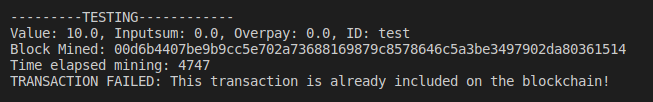
\includegraphics[width=1\linewidth]{images/check1.png}    
    \caption
    {
        This figure shows the program output when running the test to see if a transaction has already been included
        on the blockchain. This shows that program recognised this and did not proceed to adding the transaction to a 
        block.
    }
    % use the notation fig:name to cross reference a figure
    \label{fig:check1} 
\end{figure}

This resulted in the output of "TRANSACTION FAILED: This transaction is already included on the blockchain!" and as
a result the transaction did not make it through the nodes checks and was not added to the blockchain [\ref{fig:check1}].

The second test required making specialised transaction output objects to feed first into an honest transaction that
would be added to the blockchain. Then those same outputs would be fed into a second transaction to emulate a
transaction attempting to spend outputs that have already been consumed.

%Image of result
\begin{figure}[!ht]
    \centering
    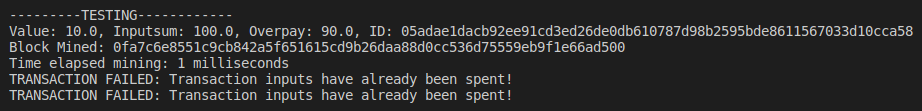
\includegraphics[width=1\linewidth]{images/inputsspent.png}    
    \caption
    {
        This figure shows the program output when attempting to create a transaction that uses transaction inputs
        that have already been consumed by a different transaction. The node scans the blockchain and disregards the
        invalid transaction and does not flood the transaction through the network.
    }
    % use the notation fig:name to cross reference a figure
    \label{fig:inputsspent}
\end{figure}

This resulted in the program outputting "TRANSACTION FAILED: Transaction inputs have already been spent!" and
therefor the node disgards the transaction, does not add the transaction to its current block, and does not flood
the transaction to other nodes [\ref{fig:inputsspent}].

The final check can be evaluated by first setting the max number of transactions in a block to a number higher than
1 to make sure that the block will not be mined before the next transaction arrives. Next an honest transaction is 
created and added to a block by a node. Then we will try to send the same transaction again to the same node. This
should trigger the test to fail.

%Image of result
\begin{figure}[!ht]
    \centering
    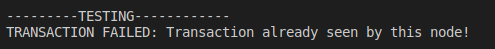
\includegraphics[width=1\linewidth]{images/seenbynode.png}    
    \caption
    {
        This figure shows the program output when running the test designed to add a transaction to a node more than
        once. The node scans through its list of transactions and catches the duplicate and disgards the transaction.
    }
    % use the notation fig:name to cross reference a figure
    \label{fig:seenbynode} 
\end{figure}

This resulted in the output "TRANSACTION FAILED: Transaction already seen by this node!" meaning the duplicate
transaction was caught and not flooded to any other nodes or added to the block a second time [\ref{fig:seenbynode}].

%Show log output from tests
\subsection{Analysis and conclusion}
%Nature of scope means that double spending may occur as number of transactions are low and so are nodes and blocks
%This is the same as bitcoin etc though and would be correct on a larger scale.
The results from these tests show that the blockchain is resistant to these single attempts to induce a double spend
attack. The first test shows how if someone were to add a transaction to the blockchain more than once they would
be stopped by the node evaluating the transaction before it is added to any blocks. The second test shows how if
someone were trying to profit by using transaction inputs that have already been consumed, maybe to dublicate a
transaction they have already made, they are also stopped by the node evaluating the transaction. The final test
shows how if someone tried to create a transaction and then before the transaction was added to a block, add the same
exact transaction to the same block in an attempt to duplicate the transaction, they would be stopped by the node.

These tests show that the network is secure against most double-spend attacks however the network is succeptable
along with most real cryptocurrencies to double spend exploitation in fringe cases. This however is a design feature
that is common in more real cryptocurrencies like Bitcoin (REFERENCE) as the scale would need to be very small for these
cases to occur. The scale of this project does mean that sometimes transactions can be created and then other transacations
can be created that use the same inputs before they are consumed by the first transaction. This issue is nullified 
at higher mining difficulty times. This is a non-factor in real world cryptocurrencies as mining is in the order of 
minutes not milliseconds however this project requires fast mining times as the test harness is being run on a singular
machine rather than many nodes with more collective compuational power.

\section{Does the cryptocurrency prevent Sybil attacks?}
A sybil attack is the act of taking over a system by forging multipe identities (REFERENCE). The name comes from a book
called Sybil by Flora Schreiber about a woman with dissociative identity dissorder. The idea behind a Sybil attack is to 
generate enough fake pseudonyms to gain control of the system with a majority vote power. The paper by John Douceur 
also shows that it is practically impossible to prevent a sybil attack on a peer-to-peer system (REFERENCE?) without some
form of central third party ensuring trust.

\subsection{Design}
In all cryptocurrencies this attack is mitigated using the proof system. Either proof of work, proof of stake, or any one
of the many methods of demonstrating proof. In this system this is implemented by proof of work and more specifically
the process of mining. This means that the system for voting on the direction of the blockchain is tied to computational 
power and not simply the existance of nodes. This means that if an attacker were to try to take over the network by 
forging a majority of nodes they would not be able to without also controlling the majority of computational power.

Bitcoin and other cryptocurrencies like the one created in this project are then able to operate under the assumtion
that there is not a majority stakeholder in the network that is malicious. This is both because it is unlikely there will
ever be a majority of computational power held by one user and also because even in there was it would be in the best 
interest of that user to remain an honest node.

The mining mechanism in this project is executed by nodes on a block when they recieve enough valid transactions to
fill a block [\ref{lst:mining}].

\begin{lstlisting}[language=java, float=h, caption=
    {
        This snippet of code shows the process of finding a hash that fits within a specified target range (hash starting
        with set number of 0s). Each loop tried a new hash by incrementing the nonce before calculating a hash. This 
        function proves that a node has expended computational power before appending to the blockchain preventing sybil
        attacks.
    }
    , label=lst:mining]
    public boolean mineBlock(int difficulty) {
        String target = new String(new char[difficulty]).replace('\0', '0');
        int nonce = 0; 
        String newHash = hash;
		while(!(newHash.substring( 0, difficulty).equals(target))) {
            nonce ++;
			newHash = calculateHash(nonce);
        }
        return true;
    }
\end{lstlisting}

This evaluation will test this function by showing that this block mining function effectivly finds a hash that fits 
within a specified range depending on the difficulty. This will demonstrate that a certain amount of computational
power must be used in order to mine a block. This will be tested using a range of different difficulties and the time
elapsed for each bock to be mined will be taken. This will show how the difficulty effects how the computational power 
required to mine a block.



\subsection{Results}
The results from these tests are displayed below [\ref{fig:avgBar}] and [\ref{fig:fulldatascatter}]. For each 
difficulty setting from 1 to 5, 20 data points were taken measuring the time elapsed during the mining of
a block. The block in question contained 10 transactions sending 100 coins to 10 different wallets. This block
remained the same for each measurement. Each measurement was run on the same laptop with the same environment
set up and no other programs running.

The first graph shows the mean of the 20 data points measured for each difficulty and how they increase relative
to the increase in difficulty level.

The second graph shows the full picture including all 100 total data points as a scatter plot. There is a logarithmic
scale on the Y axis to give a clear picture of the different scales for each difficulty.

\begin{figure}[!ht]
    \centering
    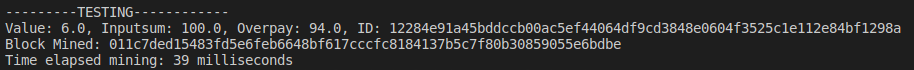
\includegraphics[width=1\linewidth]{images/check2.png}    
    \caption
    {
        This figure shows the program output during normal process when a block is being mined. Here the transaction
        details for the block, the block hash that was mined, and the time taken to complete the mining are displayed.
    }
    % use the notation fig:name to cross reference a figure
    \label{fig:check2} 
\end{figure}

\begin{figure}[!ht]
    \centering
    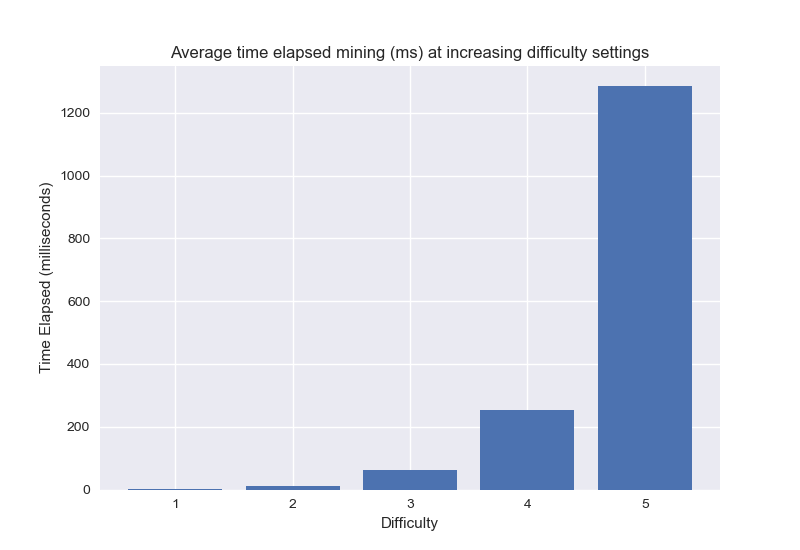
\includegraphics[width=1\linewidth]{images/avgBar.png}    
    \caption
    {
        This bar chart shows the average time elapsed in milliseconds of the block mining function for one block.
        As the difficulty increases the time elapsed grows exponentially from less than 1ms to over 1200ms. This
        demonstrates how the mining process can demonstrate different levels of computational power expended by
        nodes.
    }
    % use the notation fig:name to cross reference a figure
    \label{fig:avgBar} 
\end{figure}

\begin{figure}[!ht]
    \centering
    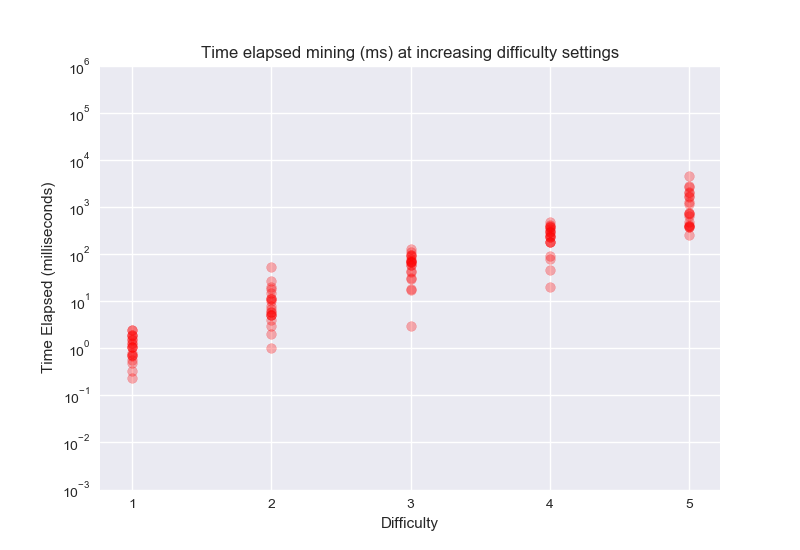
\includegraphics[width=1\linewidth]{images/fulldatascatter.png}    
    \caption
    {
        This scatter graph presents the full data set for each difficulty setting showing how long in milliseconds
        the mining process elapsed. The logarithmic scale for time elasped demonstrates clearly how the difficulty
        increasing causes the time elapsed to grow exponentially. This shows how the difficulty increasing causes
        nodes to expend exponentially more computational power in order to add blocks to the blockchain.
    }
    % use the notation fig:name to cross reference a figure
    \label{fig:fulldatascatter} 
\end{figure}

\subsection{Analysis and conclusion}
The results from testing the mining system of the show how the mining system developed for the project effectivly
demonstrates the expendature of computational power. This is clear by the increase in time elapsed increasing as the
control vairable of mining difficulty is increased. This means that the progam is effective at preventing a sybil attack
as in order to influence the blockchain an attacker would have to expend computation power and time in order to complete
the proof of work stage.

The results show only the change in time elapsed from difficulties one to five however it is safe to assume that the
exponential increase would contiue as the difficulty increases which would make it easy to adjust depending on the
size of the network much like how Bitcoin and other cryptocurrencies work (REFERENCE).

The second graph [\ref{fig:fulldatascatter}] has a logarithmic scale for time elasped better showing how the 
time increases proportionally relative to the difficulty.


\section{Is the blockchain secure?}
This final evaulation section is based on is demonstrating whether the blockchain can adapt and resist an attempt to 
alter previous transactions in the blockchain. The purpose of a blockchain is to have an immutable ledger of all transactions.
This means that once transactions enter the blockchain they cannot be altered or removed. This attack may be carried out
by users that wish to profit illegally. If they somehow were able to access and alter the blockchain they could increase
the value of a transaction sent to them or remove a transaction they made paying for a good or service.

It is not in the scope of this project to prevent any alterations to the blockchain data structure however the way the
network reacts to any changes is secure. Before mining a block, a node checks the validity of the blockchain and if it
has been altered in any way it is designed to stop and switch to a different blockchain that is valid. This way, if an
attacker managed to alter a blockchain it would fall out of use by any nodes that were using the blockchain and would
not be continued to be appended to thus rendering the attack ineffective.
\subsection{Design}
In the normal running of the project the test harness is not designed to perform attacks on the blockchain by altering
previous transactions. This means that this will be tested instead by the main function. Some transactions will first
be created between wallets and then added to blocks and mined to then be added to the blockchain. Once this has happened,
One of the transactions from the blocks will attempt to be altered. This will be implemented using a temporary function
added to the Transaction class which will allow the changing of the value of a transaction. This should alter the 
blockchain and so will cause nodes in the future to abandon this blockchchain infavour of a valid chain.

\subsection{Results}
The results of the test can be seen in [\ref{fig:check3}] where the output log from the program is shown. This shows
how the network reacts to a block being altered after it is added to the blockchain.

\begin{figure}[!ht]
    \centering
    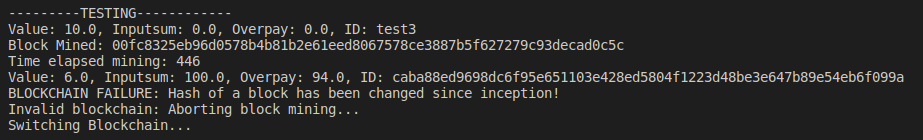
\includegraphics[width=1\linewidth]{images/check3.png}    
    \caption
    {
        This figure shows the program output when running the test designed to alter a block after it has been added
        to the blockchain. It details the first valid transaction and then it shows when a second transaction is being
        added the node recognises that the blockchain is no longer valid. The node stops what it is doing and looks
        to switch to a different valid blockchain.
    }
    % use the notation fig:name to cross reference a figure
    \label{fig:check3} 
\end{figure}

\subsection{Analysis and conclusion}
The results from this test show that the network is capable of withstanding such an attack attempting to alter previous
attributes like transactions or blocks on the blockchain. The blockchain does not prevent the actual attempt to alter
previous tranasctions as this would be out of scope and generally not necessary. Instead the network is able to recover
by checking the blockchain is valid before any changes are made. This is where the node recognises the blockchain is
incorrect and decides to scan its nearby neighbors for an alternate blockchain to try to append to. This is the safe
option and ensures that the blockchain is immutable and transactions cannot be changed once added to it. Within the
scope of this project these tests are sufficient to label the blockchain as secure and this goal as achieved.


\section{Requirements Validation}

\subsubsection{Tamperproof Ledger:}
As demonstrated by the third test in the evaluation, the blockchain that was created functioned correctly and the nodes
prevented any attempts to alter that blockchain from affecting the network. The blockchain was distributed as a version
was held by each node on the network and the nodes collectivly maintain a correct copy. This satisfies the requirement of creating a
tamper-proof distrobuted ledger.
\subsubsection{Consensus Mechanism:}
The consensus mechanism created for this project allows for nodes to maintain a list of nearby nodes in order to send
new valid transactions they recieve. This allows transactions to flood through the whole network and for all nodes to
work on adding transactions to the blockchains. This implementation satisfies the requirement of a consensus mechanism.
%SECURE consensus mechanism
\subsubsection{Proof of Work}
The proof of work system implemented in this project is seen in the second test of the evaluation to be effective. It
correctly loops through different block hashs until a hash is found within a target range. This system effectivly provided a way for nodes to present
proof that they have expended compuational power in order to add to the blockchain and maintain the honesty of the 
network.
\subsubsection{Mining Incentive \& difficulty}
The difficulty of the mining was determined by a variable which changed the target range required for nodes to hash
blocks into. This was condensed into a single variable and made it easy to modulate to control the time required to 
mine a block. This satisfies the requirement of adding a difficulty controller to the mining mechanism. Unfortunately
the program does not include the functionality for sending incentive back to nodes that mine a block. As a result the
total amount of coins in the network would never change unless new coins are manually created. In a real world scenario
this would collapse the currency as there would be no incentive to mine blocks and therefor the blockchain would either
not be appended to or run the risk of malicious nodes adding whatever transactions they wanted to the blockchain. This
means the requirement for mining incentives was not met.
\subsubsection{Merkle Tree}
In this implementation the transactions inside blocks were made to be stored using a Merkle tree structure meaning
all transactions were stored as their hash values as leaf nodes and ever branch node in the tree was the combined hash
of its two children. This provided an easy way for nodes to scan through the block and make sure that no transactions
had been altered as if there had been any alterations then the root hash would have to have been changed. This means
that the requirement of storing transactions within blocks in the Merkle tree structure was satisfied.
\subsubsection{Currency Splitting}
The project allows for users to send currency that is a smaller demonination that their current transaction inputs. This
works by sending the full transaction input and then sending the overpay back to the sender. This satisfies the 
requirement of splitting wallet currency down. 
\subsubsection{Storage Improvements}
The final requirement that was set out in the analysis section was the feature of allowing nodes to only store the
hash values inside blocks in the blockchain. This would allow nodes to save a significant amount of storage space as
they would not have to store the actual transaction objects. This feature was given a high priority and was a 
non-functional requirement and as such was not implemented in this project due to time constraints.

\section{Limitaitons}
A limitation that the project had was the issues with the scale of the project. The nature of cryptocurrencies is
that of a wide scale with many users and nodes ensuring the quality of the system. Having the test harness of this
project being run on a singular machine made having difficult and time consuming mining impossible. This lead to some
double spending issues when using small amounts of nodes and transaction. This is not a design flaw and had the project
been run on a powerful machine or the test harness being run on a network of machines it would work correctly.
%Block Size Problem (Double Spending at low user numbers)

\section{Summary}
This section evaluated how well the project satisfied the goal of being secure. The three tests that were carried out
were demonstrated and the results were shown along with some analysis why the tests prove that the system is secure.

%==================================================================================================================================
\chapter{Conclusion}
So far this paper has presented the aims and motivations for the project, how these aims were translated into functional
and non-functional requiremnets. Then the design of the cryptocurrency was presented showing how key features were examined
and planned. This section was followed by the concrete implementation methods which demonstrated how the designs were 
executed and giving light to important technical challanges that were overcome. The evaluation followed giving evidence
to show if the project was successfull at answering the main goals of the project. To conclude, a summary of the whole 
project is given.

\section{Summary}
%Summarise the whole project for a lazy reader who didn't read the rest (e.g. a prize-awarding committee).
%You should be addressing the general problem you introduced in the
%Introduction.        
%Include summary of concrete results (``the new compiler ran 2x
%faster'')
The overall goal for this project was to demonstrate the security of a basic cryptocurrency. This goal was broken down
into concrete goals for designing the cryptocurrency. First, a distributed peer-to-peer immutable ledger was created 
in order to keep a secure method of transaction history. A proof of work system was created in order to have nodes
demonstrate the expendature of computational power before adding to the blockchain. This is implemented as a mining
mechanism where node have to hash a block along with a nonce until the result is within a specified target range. A
consensus mechanism was added so nodes on the network do not have to store the address of every other node in the network
but transactions can still be flooded throughout the network and added to any blocks. Transactions within blocks are
stored using the Merkle tree strucutre in order to make the process of verifying a block much faster for nodes as they
only have to scan the root hash, not each individual transaction.

After the project was created an evauation was performed in order to see how well the cryptocurrency provided an answer
to the goal of the project. The evaluation was centered on showing that the cryptocurrency is secure and resistant to 
different types of attack that are likely to occur to a blockchain network. The evaulation consisted of three tests.
The first test evaluated how well the network resisted double-spend attacks where an attacker could add more than one
of the same transaction to the blockchain. The tests showed that the project correctly identifies these attacks and
prevents them from being included on the blockchain. The second test was designed to evaulate how the program might
deal with a Sybil attack. The project demonstrated the effectiveness of the proof of work mining mechanism. The test 
showed the time elapsed for mining a block depending on the difficulty setting. This shows how the mining mechanism 
correctly takes longer as the difficulty increases and makes it clear that nodes have to show proof of work before
adding to the blockchain. The final test aimed to evaluate how the program deals with an alteration made to a block
that has already been added to a block. The project effectivly recognised an alteration with the blockchain and 
nodes did not append to that blockchain but instead looked for a different valid blockchain to continue working on.

The cryptocurrency effectivly and securely met almost all of the requirements set at the begining of the project. It
satisfied the goals of creating a secure and robust cryptocurrency.


\section{Future Work}
%Indicate what future work could be done, but remember: you
%won't get credit for things you haven't done.
There are many different avenues that could be explored for adding to the cryptocurrency created in this project. 
Largely these improvements would be new features and not additions that would alter or improve the security of the
network. One example would be the inclusion of scripts within transaction much like Bitcoin (REFERENCE). This would a
allow for transactions to include more substance and accomplish more complex goals than just sending currency from 
one wallet to another. This could be incorperating escrow transactions or transactions that are addressed to more than
one recipient or other smart contracts (REFERENCE book).

Another place for future work could be in the network set up. Currently when a node is created it is part of the
network forever. In the real world it is likely that nodes get abandoned or shut down. Future work could allow for 
nodes to expire and be released from the network if they don't contribute to the network for a specified amount of time.

%==================================================================================================================================
%  APPENDICES  

\begin{appendices}

\chapter{Appendices}

\section{Test Code}
As the tests are not included in the main class of the project as they conflicted with the test harness, they were implemented
in a separate branch of the project. As such they are included here.

\begin{lstlisting}[language=java, float=h
    , label=lst:testCode]
    
\end{lstlisting}

\section{Mining Test Results}
\begin{table}[!ht]
    \centering
    \rowcolors{2}{}{gray!3}
    \begin{tabular}{ccccc}
    \hline
    \multicolumn{5}{c}{\textbf{Difficulty Setting}}                \\
    \textbf{1} & \textbf{2} & \textbf{3} & \textbf{4} & \textbf{5} \\ \hline
    1.300      & 53         & 45         & 180        & 2845       \\
    1.922      & 7          & 18         & 486        & 400        \\
    0.686      & 5          & 30         & 373        & 708        \\
    0.238      & 12         & 73         & 91         & 4545       \\
    1.249      & 20         & 70         & 308        & 1185       \\
    0.563      & 11         & 59         & 185        & 424        \\
    2.489      & 11         & 112        & 374        & 379        \\
    2.415      & 27         & 95         & 297        & 258        \\
    0.491      & 5          & 60         & 236        & 761        \\
    1.052      & 6          & 96         & 351        & 403        \\
    1.908      & 1          & 81         & 46         & 1769       \\
    0.739      & 3          & 69         & 258        & 640        \\
    1.073      & 10         & 41         & 20         & 2046       \\
    1.082      & 5          & 3          & 240        & 479        \\
    0.332      & 4          & 91         & 423        & 2681       \\
    1.614      & 2          & 129        & 231        & 386        \\
    0.736      & 18         & 17         & 290        & 1293       \\
    1.478      & 15         & 72         & 81         & 1662       \\
    0.805      & 8          & 69         & 406        & 2078       \\
    1.873      & 6          & 32         & 185        & 753       
    \end{tabular}
    \vspace{1cm}
    \caption{
        The full data for elapsed time to mine for different difficulty settings.
    }
    \label{tab:mining}
\end{table}
\end{appendices}

%==================================================================================================================================
%   BIBLIOGRAPHY   

% The bibliography style is abbrvnat
% The bibliography always appears last, after the appendices.

\bibliographystyle{abbrvnat}

\bibliography{l4proj}
Merkle trees

Bitcoin white paper

Bitcoin and cryptocurrency technologies

https://hackernoon.com/merkle-trees-181cb4bc30b4
[IMAGE OF MERKLE TREE] 

Blockchain technology: Principles and applications Marc Pilkington

The sybil attack John Douceur

https://blockchainwolf.net/blockchain-technology/what-is-blockchain-easiest-explanation-ever/ [blockchain diagram]

https://bitcoin.org/en/blockchain-guide [Transaction diagram]

\end{document}
